\documentclass[11pt,a4paper]{article}
\usepackage[margin=1in, headheight=14pt]{geometry}
\usepackage{amsfonts,amsmath,amssymb,suetterl}
\usepackage{lmodern}
\usepackage[T1]{fontenc}
\usepackage{fancyhdr}
\usepackage{float}
\usepackage[utf8]{inputenc}
\usepackage{fontawesome}
\usepackage{enumerate}
\usepackage{xcolor}
\usepackage{hyperref}
\usepackage{tikz}
\usepackage{nicefrac}
\usepackage{subcaption}
\usepackage{physics}
\usepackage{mathtools}
\usepackage{adjustbox}

\DeclareUnicodeCharacter{2212}{-}

\usepackage{mathrsfs}
\usepackage[nodisplayskipstretch]{setspace}

\setstretch{1.5}
\renewcommand{\footrulewidth}{0pt}

\pagestyle{fancy}
\fancyhead[R]{Problem Sheet 4}
\fancyhead[L]{MA202: Differential Equations}

\parindent 0ex
\setlength{\parskip}{1em}
\raggedbottom

\begin{document}
	\begin{center}
		\textbf{Problem Sheet 4}
	\end{center}
	%
	\begin{enumerate}
		\item Find the general solution of the given system of equations:
		\begin{align*}
			& \text{(A)}\qquad \vb{x}^\prime =
			\begin{pmatrix}
				1 & -i\\
				i & 1
			\end{pmatrix}\vb{x};\\
			%
			&	\text{(B)}\qquad \vb{x}^\prime=
			\begin{pmatrix}
				2 & 2+i\\
				-1 & -1-i
			\end{pmatrix}\vb{x};\\
			%
			& \text{(C)}\qquad \vb{x}^\prime =
			\begin{pmatrix}
				1 & 1 & 2\\
				1 & 2 & 1\\
				2 & 1 & 1
			\end{pmatrix}\vb{x}.
		\end{align*}
		%
		\item Find the general solution of the given system of equations in terms of real-valued functions:
		\begin{align*}
			& \text{(A)}\qquad \vb{x}^\prime =
			\begin{pmatrix}
				3 & 4\\
				-2 & -1
			\end{pmatrix}\vb{x};\\
			%
			& \text{(B)}\qquad \vb{x}^\prime =
			\begin{pmatrix}
				2 & 1\\
				-5 & -1
			\end{pmatrix}\vb{x}. 
		\end{align*}
		%
		\item For the linear systems below determine the eigenvalues in terms of the parameter $\alpha$ and find the critical value or values of $\alpha$ where the qualitative nature of the phase portrait for the system changes. Then draw/sketch a phase portrait for a value of $\alpha$ slightly below, and for another value slightly above, each critical value:
		\begin{align*}
			&\text{(A)}\qquad \vb{x}^\prime =
			\begin{pmatrix}
				\alpha & -1\\
				1 & \alpha
			\end{pmatrix}\vb{x};\\
			%
			&\text{(B)}\qquad \vb{x}^\prime =
			\begin{pmatrix}
				0 & -5\\
				1 & \alpha
			\end{pmatrix}\vb{x}.
		\end{align*}
		%
		\item Find the fundamental matrix $\Phi(t)$ for the given system of equations below, satisfying $\Phi(0) = \vb{I}$:
		\begin{align*}
			&\text{(A)}\qquad \vb{x}^\prime = 
			\begin{pmatrix}
				3 & 2\\
				-2 & -2
			\end{pmatrix}\vb{x}\\
			%
			&\text{(B)}\qquad \vb{x}^\prime
			\begin{pmatrix}
				1 & 4\\
				1 & -2
			\end{pmatrix}\vb{x}.
		\end{align*}
		%
		\item * The \textit{method of successive approximations} can also be applied to systems of equations. For example, consider the initial value problem
		\begin{equation}
			\vb{x}^\prime = \vb{Ax},\qquad \vb{x}(0) = \vb{x}^0,
		\end{equation}
		where $\vb{A}$ is a constant matrix and $\vb{x}^0$ is a prescribed vector.\\
		(A) Assuming that a solution $\vb{x} = \phi(t)$ exists, show that it must satisfy the integral equation
		\begin{equation}
			\phi(t) = \vb{x}^0 + \int^t_0 \vb{A}\phi(s)ds.
		\end{equation}
		(B) Start with the initial approximation $\phi^{(0)}(t) = \vb{x}^0$ . Substitute this expression for $\phi(s)$ in the right side of Eq. (2) and obtain a new approximation $\phi^{(1)}(t)$. Show that
		\begin{equation}
			\phi^{(1)}(t) = (\vb{I} + \vb{A}t)\vb{x}^0.
		\end{equation}
		(C) Repeat this process and thereby obtain a sequence of approximations $\phi^{(0)},\ \phi^{(1)},\ \phi^{(2)},$ $\ldots,\ \phi^{(n)},\ \ldots$ . Use an inductive argument to show that
		\begin{equation}
			\phi^{(n)}(t) = \left(\vb{I} + \vb{A}t + \vb{A}^2\frac{t^2}{2!} + \ldots + \vb{A}^n\frac{t^n}{n!}\right)\vb{x}^0.
		\end{equation}
		(D) Let $n \to \infty$ and show that the solution of the initial value problem (1) is
		$$
		\phi(t) = \exp(\vb{A}t)\vb{x}^0.
		$$
		\item * Find the solution of the given initial value problems and sketch the trajectory of the solution in the $x_1x_2$-plane\footnote{This question is based on the bookwork/self-study material of Section 7.8 (Repeated Eigenvalues) of the main textbook by Boyce and DiPrima}:
		\begin{align*}
			&\text{(A)}\qquad \vb{x}^\prime =
			\begin{pmatrix}
				1 & -4\\
				4 & -7
			\end{pmatrix}\vb{x},\quad \vb{x}(0) = 
			\begin{pmatrix}
				4\\
				2
			\end{pmatrix};\\
			%
			&\text{(B)}\qquad \vb{x}^\prime =
			\begin{pmatrix}
				3 & -1\\
				9 & -3
			\end{pmatrix}\vb{x},\quad \vb{x}(0) =
			\begin{pmatrix}
				2 \\
				4
			\end{pmatrix}.
		\end{align*}
		%
		\item Find the general solution of the given system of equations:
		\begin{align*}
			&\text{(A)}\qquad \vb{x}^\prime =
			\begin{pmatrix}
				2 & 3\\
				-1 & -2
			\end{pmatrix}\vb{x} + 
			\begin{pmatrix}
				e^t\\
				t
			\end{pmatrix};\\
			%
			\displaybreak
			&\text{(B)}\qquad \vb{x}^\prime =
			\begin{pmatrix}
				2 & 1\\
				-5 & -2
			\end{pmatrix}\vb{x} + 
			\begin{pmatrix}
				-\cos t\\
				\sin t
			\end{pmatrix};\\
			%
			&\text{(C)}\qquad \vb{x}^\prime =
			\begin{pmatrix}
				4 & 8\\
				-2 & -4
			\end{pmatrix}\vb{x} + 
			\begin{pmatrix}
				t^{-3}\\
				-t^{-2}
			\end{pmatrix}.
		\end{align*}
		%
		\item For the linear systems below, classify the critical point $(0, 0)$ as to type and determine whether it is stable, asymptotically stable, or unstable (you may find useful the information summarised in Table 1 below):
		\begin{align*}
			&\text{(A)}\qquad \vb{x}^\prime = 
			\begin{pmatrix}
				3 & 2\\
				-2 & -2
			\end{pmatrix};\\
			%
			&\text{(B)}\qquad \vb{x}^\prime =
			\begin{pmatrix}
				5 & 3\\
				-1 & 1
			\end{pmatrix}\vb{x};\\
			%
			&\text{(C)}\qquad \vb{x}^\prime = 
			\begin{pmatrix}
				1 & 4\\
				-4 & -7
			\end{pmatrix}\vb{x}.
		\end{align*}
		%
		\item Consider the linear system
		\begin{align*}
			& \frac{dx}{dt} = a_{11}x + a_{12}y,\\
			& \frac{dy}{dt} = a_{21}x + a_{22}y,
		\end{align*}
		%
		\begin{table}[H]
			\centering
			\begin{tabular}{ |l|l|l| } 
			 \hline
			 \textbf{Eigenvalues} & \textbf{Type of Critical Point} & \textbf{Stability}\\
			 \hline
			 \hline
			 $r_1>r_2>0$ & Node & Unstable \\
			 \hline
			 $r_1 < r_2 < 0$ & Node & Asymptotically Stable \\
			 \hline
			 $r_2 < 0 < r_1$ & Saddle Point & Unstable \\ 
			 \hline
			 $r_1 = r_2 > 0$ & Proper or Improper Node & Unstable \\
			 \hline
			 $r_1 = r_2 < 0$ & Proper or Improper Node & Asymptotically Stable \\
			 \hline
			 $r_1,r_2 = \lambda \pm i\mu$ & Spiral Point &  \\
			 
			 $\lambda > 0$ &  & Unstable \\
			 
			 $\lambda < 0$ &  & Asymptotically Stable \\
			 \hline
			 $r_1 = i\mu, r_2 = -i\mu$ & Center & Stable \\
			 \hline
			\end{tabular}
			\caption{ Stability Properties of Linear Systems $\vb{x}^\prime = \vb{Ax}$ with $\det(\vb{A} - r\vb{I}) = 0$ and $\det \vb{A} \neq 0$.}
		\end{table}
		%
		\begin{figure}[H]
			\centering
			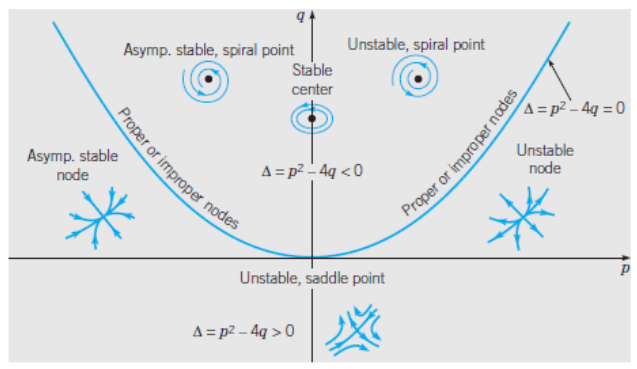
\includegraphics[width=0.45\textwidth]{figure/3_fig1.PNG}
			\caption{Stability diagram (see Question 11).}
		\end{figure}
		%
		where $a_{11},\ a_{12},\ a_{21}$ and $a_{22}$ are real constants. Let $p = a_{11} + a_{22},\ q = a_{11}a_{22} - a_{12}a_{21}$, and $\Delta = p^2 - 4q$. Observe that $p$ and $q$ are the trace and determinant, respectively, of the coefficient matrix of the given system. Show that the critical point $(0, 0)$ is a (see Fig. 1)
		\begin{enumerate}[(A)]
			\item Node if $q > 0$ and $\Delta \geq 0$;
			\item Saddle point if $q < 0$;
			\item Spiral point if $p \neq 0$ and $\Delta < 0$;
			\item Center if $p = 0$ and $q > 0$.
		\end{enumerate}
		\textbf{Hint:} These conclusions can be obtained by studying the eigenvalues $r_1$ and $r_2$. It may also be helpful to establish, and then to use, the relations $r_1r_2 = q$ and $r_1 + r_2 = p$.
	\end{enumerate}
\end{document}